\documentclass{beamer}
\usepackage{tikz}
\usetikzlibrary{arrows,positioning,shapes,calc}
\usepackage{amsmath,amssymb}
\usepackage{booktabs}

% Clean, professional presentation styling
\usetheme{default}
\usecolortheme{default}
\setbeamertemplate{navigation symbols}{} % Remove navigation symbols
\setbeamercolor{structure}{fg=blue!80!black}
\setbeamercolor{titlelike}{parent=structure,fg=blue!80!black}
\setbeamercolor{item}{fg=blue!80!black}

\begin{document}

% Slide 1: Hidden Markov Models
\begin{frame}{Hidden Markov Models}
    \centering
    \vfill
    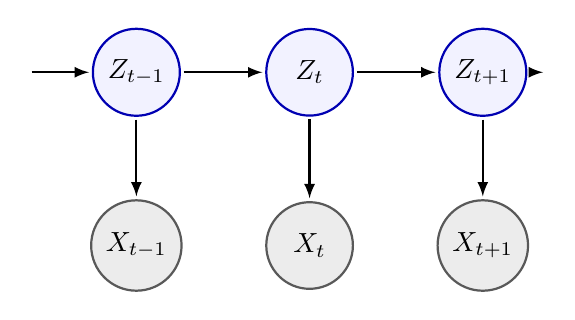
\begin{tikzpicture}[
        node distance=2.2cm,
        latent/.style={circle, draw=blue!70!black, fill=blue!5, thick, minimum size=11mm},
        observed/.style={circle, draw=gray!70!black, fill=gray!15, thick, minimum size=11mm},
        arrow/.style={-latex, thick, shorten >=1pt, shorten <=1pt}
    ]
        % Latent nodes
        \node[latent] (z1) {$Z_{t-1}$};
        \node[latent, right of=z1] (z2) {$Z_t$};
        \node[latent, right of=z2] (z3) {$Z_{t+1}$};
        
        % Observed nodes
        \node[observed, below of=z1] (x1) {$X_{t-1}$};
        \node[observed, below of=z2] (x2) {$X_t$};
        \node[observed, below of=z3] (x3) {$X_{t+1}$};
        
        % Latent transitions
        \draw[arrow] (z1) -- (z2);
        \draw[arrow] (z2) -- (z3);
        \draw[arrow] (z1.west)++(-0.8cm,0) -- (z1);
        \draw[arrow] (z3) -- ++(0.8cm,0);
        
        % Emission transitions
        \draw[arrow] (z1) -- (x1);
        \draw[arrow] (z2) -- (x2);
        \draw[arrow] (z3) -- (x3);
    \end{tikzpicture}
    \vfill
\end{frame}

% Slide 2: Deep Latent Gaussian Models (DLGMs)
\begin{frame}{Deep Latent Gaussian Models (DLGMs)}
    \centering
    \vfill
    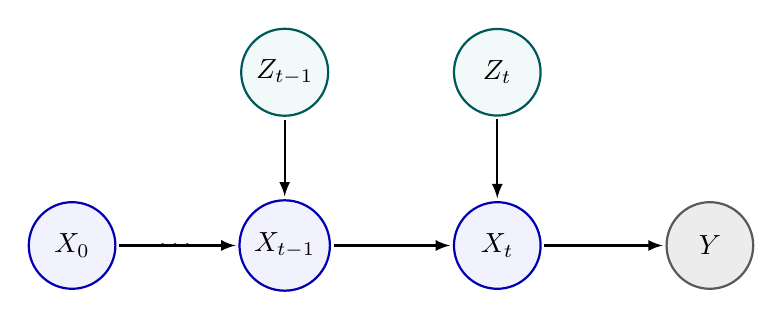
\begin{tikzpicture}[
        node distance=2.2cm,
        latent/.style={circle, draw=blue!70!black, fill=blue!5, thick, minimum size=11mm},
        noise/.style={circle, draw=teal!70!black, fill=teal!5, thick, minimum size=11mm},
        observed/.style={circle, draw=gray!70!black, fill=gray!15, thick, minimum size=11mm},
        arrow/.style={-latex, thick, shorten >=1pt, shorten <=1pt}
    ]
        % Latent state nodes
        \node[latent] (x0) {$X_0$};
        \node[latent, right of=x0, xshift=0.5cm] (x1) {$X_{t-1}$};
        \node[latent, right of=x1, xshift=0.5cm] (x2) {$X_t$};
        \node[observed, right of=x2, xshift=0.5cm] (y) {$Y$};
        
        % Noise nodes (above)
        \node[noise, above of=x1] (z1) {$Z_{t-1}$};
        \node[noise, above of=x2] (z2) {$Z_t$};
        
        % Transitions
        \draw[arrow] (x0) -- (x1);
        \draw[arrow] (x1) -- (x2);
        \draw[arrow] (x2) -- (y);
        
        % Noise injections
        \draw[arrow] (z1) -- (x1);
        \draw[arrow] (z2) -- (x2);
        
        % Dots between X0 and X(t-1)
        \path (x0) -- (x1) node [midway] {$\dots$};
    \end{tikzpicture}
    
    \vspace{1.0cm}
    \textbf{\large\textcolor{blue!80!black}{Discrete Stochastic Flow}}
    \vfill
\end{frame}

% Slide 3: Neural SDEs as the Diffusion Limit of DGLMs (I)
\begin{frame}{Neural SDEs as the Diffusion Limit of DGLMs (I)}
    \begin{columns}[c]
        \begin{column}{0.5\textwidth}
            \centering
            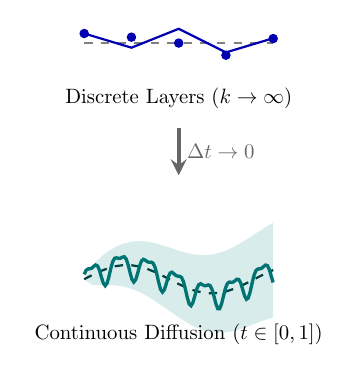
\begin{tikzpicture}[scale=0.6, every node/.style={scale=0.75}]
                % Discrete path
                \draw[gray, dashed] (0,0) -- (4,0);
                \foreach \x in {0,1,2,3,4} {
                    \filldraw[blue!70!black] (\x, {0.3*sin(\x*100) + 0.2*cos(\x*150)}) circle (2.5pt);
                }
                \draw[blue!70!black, thick] (0,0.2) -- (1, -0.1) -- (2, 0.3) -- (3, -0.2) -- (4, 0.1);
                \node[below] at (2, -0.8) {Discrete Layers ($k \to \infty$)};

                % Arrow showing limit
                \draw[->, >=stealth, line width=1.5pt, black!60] (2, -1.8) -- (2, -2.8) node[midway, right] {$\Delta t \to 0$};

                % Continuous path
                \begin{scope}[yshift=-5cm]
                    \fill[teal!15] plot[domain=0:4] (\x, {0.3*sin(\x*100) + 0.5*sqrt(\x)}) 
                                -- plot[domain=4:0] (\x, {0.3*sin(\x*100) - 0.5*sqrt(\x)}) -- cycle;
                    \draw[teal!50!black, dashed, thick] plot[domain=0:4] (\x, {0.3*sin(\x*100)});
                    \draw[teal!90!black, very thick] plot[domain=0:4, samples=100] (\x, {0.3*sin(\x*100) + 0.25*sin(\x*600) + 0.1*cos(\x*1200)});
                    \node[below] at (2, -0.8) {Continuous Diffusion ($t \in [0,1]$)};
                \end{scope}
            \end{tikzpicture}
        \end{column}
        
        \begin{column}{0.5\textwidth}
            \textbf{Diffusion Limit of DLGMs:}
            \begin{itemize}
                \item \textbf{Transition Scale}: \\
                $\mu_t \propto \Delta t$, \quad $\sigma_t \propto \sqrt{\Delta t}$
                \item \textbf{Limit SDE (It\^o)}: \\
                $dX_t = \mu(X_t, t)dt + \sigma(X_t, t)dW_t$
                \item \textbf{Continuous Depth}: \\
                Layer index $i \to$ continuous time $t \in [0, 1]$
                \item \textbf{Parametrization}: \\
                Drift $\mu$ and diffusion $\sigma$ modeled by neural networks $\mu_\theta$, $\sigma_\phi$
            \end{itemize}
        \end{column}
    \end{columns}
\end{frame}

% Slide 4: Neural SDEs as the Diffusion Limit of DGLMs (II)
\begin{frame}{Neural SDEs as the Diffusion Limit of DGLMs (II)}
    \begin{columns}[c]
        \begin{column}{0.5\textwidth}
            \centering
            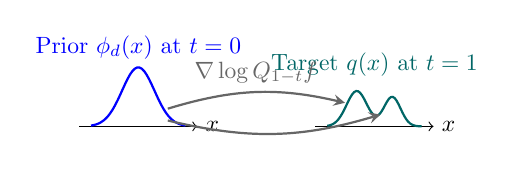
\begin{tikzpicture}[scale=0.75, every node/.style={scale=0.85}]
                % Prior Axis
                \draw[->] (-2.5,0) -- (-0.5,0) node[right] {$x$};
                \draw[blue, thick, domain=-2.3:-0.7, samples=40] plot (\x, {1.0*exp(-(\x+1.5)^2/0.15)});
                \node[blue, above] at (-1.5, 1.0) {Prior $\phi_d(x)$ at $t=0$};
                
                % Target Axis
                \draw[->] (1.5,0) -- (3.5,0) node[right] {$x$};
                \draw[teal!80!black, thick, domain=1.7:3.3, samples=50] plot (\x, {0.6*exp(-(\x-2.2)^2/0.06) + 0.5*exp(-(\x-2.8)^2/0.04)});
                \node[teal!80!black, above] at (2.5, 0.7) {Target $q(x)$ at $t=1$};
                
                % Transport paths
                \draw[->, >=stealth, thick, bend left=15, black!60] (-1.0, 0.3) to node[midway, above] {$\nabla \log Q_{1-t}f$} (2.0, 0.4);
                \draw[->, >=stealth, thick, bend right=15, black!60] (-1.0, 0.1) to (2.6, 0.2);
            \end{tikzpicture}
            
            \vspace{0.4cm}
            \small
            \textbf{Heat Semigroup Operator}: \\
            $Q_t f(x) = \mathbb{E}_{Z \sim \mathcal{N}(0, \mathbb{I})}[f(x + \sqrt{t}Z)]$
        \end{column}
        
        \begin{column}{0.5\textwidth}
            \textbf{Expressiveness \& Parameter Efficiency:}
            \begin{itemize}
                \item \textbf{Drift-Only Expressiveness}: \\
                Setting $\sigma \equiv \mathbb{I}_d$ is sufficient to target any smooth distribution $q(x) = f(x)\phi_d(x)$.
                \item \textbf{F\"ollmer Drift}: \\
                SDE path connects prior to target exactly:
                \[ dX_t = \nabla \log Q_{1-t} f(X_t) dt + dW_t \]
                \item \textbf{Weight Sharing}: \\
                A single neural network $\hat{f}(x, t; \theta)$ models the drift across all time $t$. No layer-specific weights needed.
            \end{itemize}
        \end{column}
    \end{columns}
\end{frame}

% Slide 5: Latent SDEs (I)
\begin{frame}{Latent SDEs: Path-Space Variational Inference}
    \begin{columns}[c]
        \begin{column}{0.5\textwidth}
            \centering
            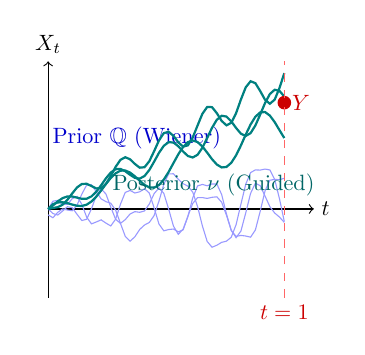
\begin{tikzpicture}[scale=0.75, every node/.style={scale=0.8}]
                % Coordinates
                \draw[->] (0,0) -- (4.5,0) node[right] {$t$};
                \draw[->] (0,-1.5) -- (0,2.5) node[above] {$X_t$};
                
                % Prior paths (starting at 0, spreading out)
                \draw[blue!40, thin] plot[domain=0:4, samples=50] (\x, {0.3*sqrt(\x)*sin(\x*300) + 0.1*sin(\x*900)});
                \draw[blue!40, thin] plot[domain=0:4, samples=50] (\x, {-0.4*sqrt(\x)*cos(\x*250) - 0.1*cos(\x*800)});
                \draw[blue!40, thin] plot[domain=0:4, samples=50] (\x, {0.2*sqrt(\x)*cos(\x*400) - 0.15*sin(\x*700)});
                \node[blue!80!black] at (1.5, 1.2) {Prior $\mathbb{Q}$ (Wiener)};
                
                % Posterior paths (guided towards Y at t=1)
                \draw[teal, thick] plot[domain=0:4, samples=50] (\x, {0.45*\x + 0.15*sqrt(\x)*sin(\x*400)});
                \draw[teal, thick] plot[domain=0:4, samples=50] (\x, {0.45*\x - 0.1*\x + 0.2*sqrt(\x)*cos(\x*300)});
                \draw[teal, thick] plot[domain=0:4, samples=50] (\x, {0.45*\x + 0.1*\x - 0.15*sqrt(\x)*sin(\x*500)});
                \node[teal!80!black] at (2.8, 0.4) {Posterior $\nu$ (Guided)};
                
                % Target / Observation Y at t=1 (x=4)
                \filldraw[red!80!black] (4, 1.8) circle (3pt) node[right] {$Y$};
                \draw[dashed, red!60] (4, -1.5) -- (4, 2.5);
                \node[red!80!black, below] at (4, -1.5) {$t=1$};
            \end{tikzpicture}
        \end{column}
        
        \begin{column}{0.5\textwidth}
            \textbf{Infinite-Dimensional Latent Space:}
            \begin{itemize}
                \item \textbf{Latent Paths}: Wiener space $\mathbf{W}$ of continuous trajectories on $t \in [0, 1]$.
                \item \textbf{Prior Measure} $\mathbb{Q}$: Probability law of standard Brownian motion.
                \item \textbf{Posterior Measure} $\nu$: Approximate posterior path distribution.
                \item \textbf{Gibbs Variational Principle}:
                \[ -\log \mathbb{P}_\theta[Y] = \inf_{\nu \in \mathcal{P}(\mathbf{W})} \Big\{ \text{KL}(\nu \parallel \mathbb{Q}) - \mathbb{E}_\nu [\log \mathbb{P}_\theta(Y \mid X_1)] \Big\} \]
            \end{itemize}
        \end{column}
    \end{columns}
\end{frame}

% Slide 6: Latent SDEs (II)
\begin{frame}{Latent SDEs: Girsanov Reparameterization}
    \centering
    \vfill
    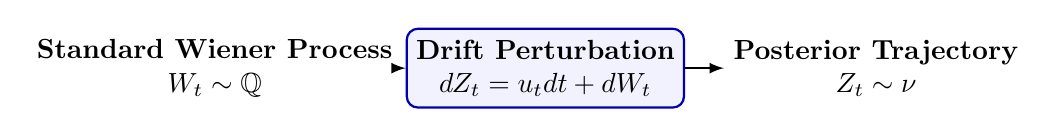
\begin{tikzpicture}[
        node distance=3cm,
        block/.style={rectangle, draw=blue!70!black, fill=blue!5, thick, rounded corners, minimum height=10mm, align=center},
        arrow/.style={-latex, thick}
    ]
        \node (w) [align=center] {\textbf{Standard Wiener Process} \\ $W_t \sim \mathbb{Q}$};
        \node[block, right of=w, xshift=1.2cm] (drift) {\textbf{Drift Perturbation} \\ $dZ_t = u_t dt + dW_t$};
        \node[right of=drift, xshift=1.2cm] (z) [align=center] {\textbf{Posterior Trajectory} \\ $Z_t \sim \nu$};
        
        \draw[arrow] (w) -- (drift);
        \draw[arrow] (drift) -- (z);
    \end{tikzpicture}
    
    \vspace{0.6cm}
    \begin{columns}[t]
        \begin{column}{0.5\textwidth}
            \textbf{Girsanov's Theorem:}
            \begin{itemize}
                \item Maps reference measure $\mathbb{Q}$ to posterior $\nu$ via control drift $u_t$.
                \item Reduces path-space KL to a simple quadratic penalty:
                \[ \text{KL}(\nu \parallel \mathbb{Q}) = \mathbb{E}_{\mathbb{Q}} \left[ \frac{1}{2} \int_0^1 \|u_t\|^2 dt \right] \]
            \end{itemize}
        \end{column}
        
        \begin{column}{0.5\textwidth}
            \textbf{Variational Free Energy:}
            \begin{itemize}
                \item Parameterize $u_t$ as $\tilde{\mu}(Y, t; \beta)$ (Neural Net).
                \item Objective to minimize:
                \[ \mathcal{F}_{\theta, \beta}(y) = \mathbb{E} \left[ \frac{1}{2}\int_0^1 \|\tilde{\mu}\|^2 dt - \log \mathbb{P}_\theta[y \mid Z_1] \right] \]
                \item \textbf{Drift-Only Control}: Posterior diffusion remains standard.
            \end{itemize}
        \end{column}
    \end{columns}
    \vfill
\end{frame}

% Slide 7: Stochastic Adjoint Method
\begin{frame}{Stochastic Adjoint Method}
    \begin{table}
        \centering
        \small
        \begin{tabular}{lccl}
            \hline
            \textbf{Method} & \textbf{Memory} & \textbf{Time} & \textbf{Key Limitation} \\ \hline
            Euler--Maruyama AD & $\mathcal{O}(L)$ & $\mathcal{O}(L)$ & Caches all states/noise in memory \\
            Forward Sensitivity & $\mathcal{O}(1)$ & $\mathcal{O}(nd^2)$ & Scale-intractable Jacobian forward pass \\
            \textbf{Stochastic Adjoint} & $\mathcal{O}(1)$ & $\mathcal{O}(L)$ & Requires invertible Stratonovich flow \\ \hline
        \end{tabular}
    \end{table}

    \vspace{0.2cm}
    \textbf{Stratonovich Backward Flow \& Adjoint System (Li et al., 2020):}
    \begin{itemize}
        \item \textbf{Stratonovich SDE} (Symmetric): \\
        $dX_t = \mu(X_t, t; \theta)dt + \sigma(X_t, t) \circ dW_t$
        \item \textbf{Backward Flow} $\psi_{s,t}(x) = X_s$: \\
        $d\psi_{s,t}(x) = -\mu(\psi_{s,t}(x), u)du - \sigma(\psi_{s,t}(x), u) \circ d\check{W}_u$ \quad ($d\check{W}_u$ is backward noise)
        \item \textbf{Adjoint SDE} ($B_{s,t}(x) = \nabla \mathcal{L}(X_t) \nabla_x \phi_{s,t}(x)$):
        \[ B_{s,t}(x) = \nabla \mathcal{L}(x) + \int_s^t \nabla \mu(\psi_{r,t}(x), r)^T B_{r,t}(x) dr + \int_s^t \nabla \sigma(\psi_{r,t}(x), r)^T B_{r,t}(x) \circ d\check{W}_r \]
        \item \textbf{On-the-fly Reconstruction}: Brownian motion reconstructed from a single seed via \textit{virtual Brownian trees}, yielding $\mathcal{O}(1)$ memory.
    \end{itemize}
\end{frame}

\end{document}
